\UC{Aggiunta nuovo prodotto}
Il venditore aggiunge un nuovo prodotto alla piattaforma, così da poter essere venduto.
\begin{itemize}
    \item \textbf{Attori primari:} venditore;
    \item \textbf{Precondizione:} il venditore si trova nella schermata di amministrazione dei prodotti e vuole aggiungere un nuovo prodotto;
    \item \textbf{Postcondizione:} il venditore ha inserito il nuovo prodotto nella piattaforma;
    \item \textbf{Scenario principale:} il venditore seleziona la funzionalità per aggiungere un nuovo prodotto e compie le seguenti azioni:
    \begin{itemize}
        \item (\actualUC.1) - Inserimento del nome del prodotto;
        \item (\actualUC.2) - Inserimento della descrizione del prodotto;
        \item (\actualUC.3) - Inserimento delle categorie del prodotto;
        \item (\actualUC.4) - Inserimento del prezzo del prodotto;
        \item (\actualUC.5) - Inserimento dello sconto percentuale al prezzo del prodotto;
        \item (\actualUC.6) - Inserimento della quantità del prodotto disponibile in magazzino;
        \item (\actualUC.7) - Inserimento delle foto del prodotto;
        \item Sceglie se aggiungere il prodotto tra quelli in evidenza tramite la funzionalità apposita;
        \item Conferma gli inserimenti e aggiunge il prodotto alla piattaforma.
    \end{itemize}
    \item \textbf{Scenari alternativi:}
	\begin{enumerate}[label=\lett]
		\item Il venditore non conferma la creazione del nuovo prodotto e di conseguenza questo non verrà aggiunto.
	\end{enumerate}
\end{itemize}

\resetSubUC

\subUC{Inserimento del nome del prodotto}
Il venditore inserisce il nome del prodotto da aggiungere.
\begin{itemize}
    \item \textbf{Attori primari:} venditore;
    \item \textbf{Precondizione:} il venditore si trova nella schermata di aggiunta di un nuovo prodotto;
    \item \textbf{Postcondizione:} il venditore ha inserito il nome del prodotto;
    \item \textbf{Scenario principale:} il venditore aggiunge il nome del prodotto da inserire;
    \item \textbf{Estensioni:} 
    \begin{enumerate}[label=\lett]
    	\item Il venditore non inserisce il nome del prodotto ed il campo dati risulta essere vuoto. In questo caso:
	    \begin{itemize}
	        \item (UC) - Viene visualizzato il messaggio di errore campo dati obbligatorio non inserito;
	        \item Viene data la possibilità al venditore di modificare il nome del nuovo prodotto inserito.
	    \end{itemize}
    	\item Il venditore inserisce un nome composto da troppi caratteri per il nuovo prodotto. In questo caso:
    	\begin{itemize}
    		\item (UC) - Viene visualizzato il messaggio di errore in caso di inserimento di un numero eccessivo di caratteri;
    		\item Viene data la possibilità al venditore di modificare il nome del nuovo prodotto inserito.
    	\end{itemize}
	\end{enumerate}
\end{itemize}

\subUC{Inserimento della descrizione del prodotto}
Il venditore inserisce la descrizione del prodotto da aggiungere.
\begin{itemize}
    \item \textbf{Attori primari:} venditore;
    \item \textbf{Precondizione:} il venditore si trova nella schermata di aggiunta di un nuovo prodotto;
    \item \textbf{Postcondizione:} il venditore ha inserito la descrizione del prodotto;
    \item \textbf{Scenario principale:} il venditore aggiunge la descrizione del prodotto da inserire;
    \item \textbf{Estensioni:}
    \begin{enumerate}[label=\lett]
    	\item Il venditore non inserisce la descrizione del prodotto ed il campo dati risulta essere vuoto. In questo caso:
    	\begin{itemize}
    		\item (UC) - Viene visualizzato il messaggio di errore campo dati obbligatorio non inserito;
    		\item Viene fornita al venditore la possibilità di modificare la descrizione del nuovo prodotto inserito.
    	\end{itemize}
        \item Il venditore inserisce una descrizione composta da troppi caratteri per il nuovo prodotto. In questo caso:
	    \begin{itemize}
    		\item (UC) - Viene visualizzato il messaggio di errore in caso di inserimento di un numero eccessivo di caratteri;
	    	\item Viene fornita al venditore la possibilità di modificare la descrizione del nuovo prodotto inserito.
	    \end{itemize}
    \end{enumerate}
\end{itemize}

\subUC{Inserimento delle categorie del prodotto}
Il venditore inserisce le categorie del prodotto da aggiungere.
\begin{itemize}
    \item \textbf{Attori primari:} venditore;
    \item \textbf{Precondizione:} il venditore si trova nella schermata di aggiunta di un nuovo prodotto;
    \item \textbf{Postcondizione:} il venditore ha inserito le categorie del prodotto;
    \item \textbf{Scenario principale:} il venditore inserisce le categorie a cui fa parte il prodotto scegliendole dalla lista di categorie disponibili nella piattaforma;
    \item \textbf{Scenari alternativi:}
    \begin{enumerate}[label=\lett]
    	\item Il venditore non ha inserito alcuna categoria e il prodotto viene automaticamente categorizzato come senza categoria.
    \end{enumerate}
\end{itemize}

\subUC{Inserimento del prezzo del prodotto}
Il venditore inserisce il prezzo a cui vendere il prodotto da aggiungere.
\begin{itemize}
    \item \textbf{Attori primari:} venditore;
    \item \textbf{Precondizione:} il venditore si trova nella schermata di aggiunta di un nuovo prodotto;
    \item \textbf{Postcondizione:} il venditore ha inserito il prezzo a cui vendere il prodotto;
    \item \textbf{Scenario principale:} il venditore inserisce il prezzo a cui vendere il prodotto;
    \item \textbf{Estensioni:}
    \begin{enumerate}[label=\lett]
    	\item Il venditore non inserisce il prezzo del prodotto ed il campo dati risulta essere vuoto. In questo caso:
    	\begin{itemize}
    		\item (UC) - Viene visualizzato il messaggio di errore campo dati obbligatorio non inserito;
    		\item Viene fornita al venditore la possibilità di aggiungere un prezzo al nuovo prodotto inserito.
    	\end{itemize}
    	\item Il venditore inserisce un prezzo minore o uguale a zero. In questo caso:
    	\begin{itemize}
    		\item (UC) - Viene visualizzato il messaggio di errore prezzo minore o uguale a zero;
    		\item Viene fornita al venditore la possibilità di aggiungere un nuovo prezzo al prodotto da inserire.
    	\end{itemize}
    \end{enumerate}
\end{itemize}

\subUC{Inserimento dello sconto percentuale al prezzo del prodotto}
Il venditore inserisce lo sconto percentuale da applicare al prezzo del prodotto da aggiungere.
\begin{itemize}
    \item \textbf{Attori primari:} venditore;
    \item \textbf{Precondizione:} il venditore si trova nella schermata di aggiunta di un nuovo prodotto;
    \item \textbf{Postcondizione:} il venditore ha inserito lo sconto percentuale da applicare al prezzo del prodotto;
    \item \textbf{Scenario principale:} il venditore inserisce lo sconto percentuale da applicare al prezzo del prodotto. In seguito il prezzo a cui vendere quel prodotto sarà scontato della percentuale applicata;
    \item \textbf{Scenari alternativi:}
    \begin{enumerate}[label=\lett]
    	\item Nel caso in cui il venditore non inserisce alcuno sconto, il prezzo non viene modificato in alcun modo.
    \end{enumerate}
    \item \textbf{Estensioni:}
    \begin{enumerate}[label=\lett]
    	\item Il venditore inserisce uno sconto maggiore di 100\%. In questo caso:
    	\begin{itemize}
    		\item (UC) - Viene visualizzato il messaggio di errore in caso di sconto maggiore di 100\%;
    		\item Viene fornita al venditore la possibilità di modificare lo sconto da applicare al nuovo prodotto.
    	\end{itemize}
    	\item Il venditore inserisce uno sconto minore di 0\%. In questo caso:
    	\begin{itemize}
    		\item (UC) - Viene mostrato un messaggio di errore che segnala lo sconto minore di 0\%;
    		\item Viene fornita al venditore la possibilità di modificare lo sconto da applicare al nuovo prodotto.
    	\end{itemize}
    \end{enumerate}
\end{itemize}

\subUC{Inserimento della quantità del prodotto disponibile in magazzino}
Il venditore inserisce la quantità disponibile attualmente in magazzino del prodotto da aggiungere.
\begin{itemize}
    \item \textbf{Attori primari:} venditore;
    \item \textbf{Precondizione:} il venditore si trova nella schermata di aggiunta di un nuovo prodotto;
    \item \textbf{Postcondizione:} il venditore ha inserito la quantità disponibile attualmente in magazzino del prodotto;
    \item \textbf{Scenario principale:} il venditore inserisce la quantità disponibile attualmente in magazzino del prodotto;
    \item \textbf{Scenari alternativi:}
    \begin{enumerate}[label=\lett]
    	\item Nel caso in cui il venditore inserisca 0 come disponibilità attuale, allora il prodotto verrà indicato come non disponibile.
    \end{enumerate}
    \item \textbf{Estensioni:}
    \begin{enumerate}[label=\lett]
    	\item Il venditore inserisce una quantità minore di 0. In questo caso:
    	\begin{itemize}
    		\item (UC) - Viene visualizzato il messaggio di errore quantità minore di 0;
    		\item Viene fornita la possibilità al venditore di modificare la quantità inserita per il nuovo prodotto.
    	\end{itemize}
    	\item Il venditore non inserisce la quantità del prodotto ed il campo dati risulta essere vuoto. In questo caso:
    	\begin{itemize}
    		\item (UC) - Viene visualizzato il messaggio di errore campo dati obbligatorio non inserito;
    		\item Viene fornita la possibilità al venditore di aggiungere la quantità inserita per il nuovo prodotto.
    	\end{itemize}
    \end{enumerate}
\end{itemize}

\subUC{Inserimento foto del prodotto}
Il venditore inserisce le foto relative al prodotto da aggiungere.
\begin{itemize}
    \item \textbf{Attori primari:} venditore;
    \item \textbf{Precondizione:} il venditore si trova nella schermata di aggiunta di un nuovo prodotto;
    \item \textbf{Postcondizione:} il venditore ha inserito le foto relative al prodotto;
    \item \textbf{Scenario principale:} il venditore inserisce al più il numero massimo di foto consentite relative al prodotto;
    \item \textbf{Estensioni:}
    \begin{enumerate}[label=\lett]
    	\item Il venditore non inserisce alcuna foto del prodotto. In questo caso:
    	\begin{itemize}
    		\item (UC) - Viene visualizzato il messaggio di errore nessuna foto inserita;
    		\item Viene fornita al venditore la possibilità di inserire altre foto relative al nuovo prodotto.
    	\end{itemize}
    	\item Il venditore seleziona un file che non è del tipo immagine. In questo caso:
    	\begin{itemize}
    		\item (UC) - Viene visualizzato il messaggio di errore il quale segnala che il file selezionato non è del tipo immagine;
    		\item Viene fornita la possibilità al venditore di cambiare i file selezionati per il nuovo prodotto.
    	\end{itemize}
    	\item Il venditore cerca di inserire più del massimo numero di foto consentite relative ad un prodotto. In questo caso:
    	\begin{itemize}
    		\item (UC) - Viene visualizzato il messaggio di errore il quale segnala il tentativo di aggiunta di più del numero massimo di foto consentite relative ad un prodotto;
    		\item Viene fornita la possibilità al venditore di rimuovere alcune foto selezionate per il nuovo prodotto da inserire.
    	\end{itemize}
    \end{enumerate}
\end{itemize}

%%%%%%%%%%%%%%%%%%%%%%%%%%%%%%%%%%%%%%%%%%%%%%%%%%%%%%%%%%%%%%%%%%%%%%%%%%%%%%%%%%%%%%%%%%%%%%%%%%%%%%%%%%%%%%%%%%%%%%%%%%%%%%%%%%%%%%%%%%%%%%%%%%%%%%%%%%%%%%%%%%%%%%%%%%%%%%%%%%%%%%%%%%%%%%

\UC{Modifica informazioni del prodotto}
% \begin{figure}[H]
%     \centering
%     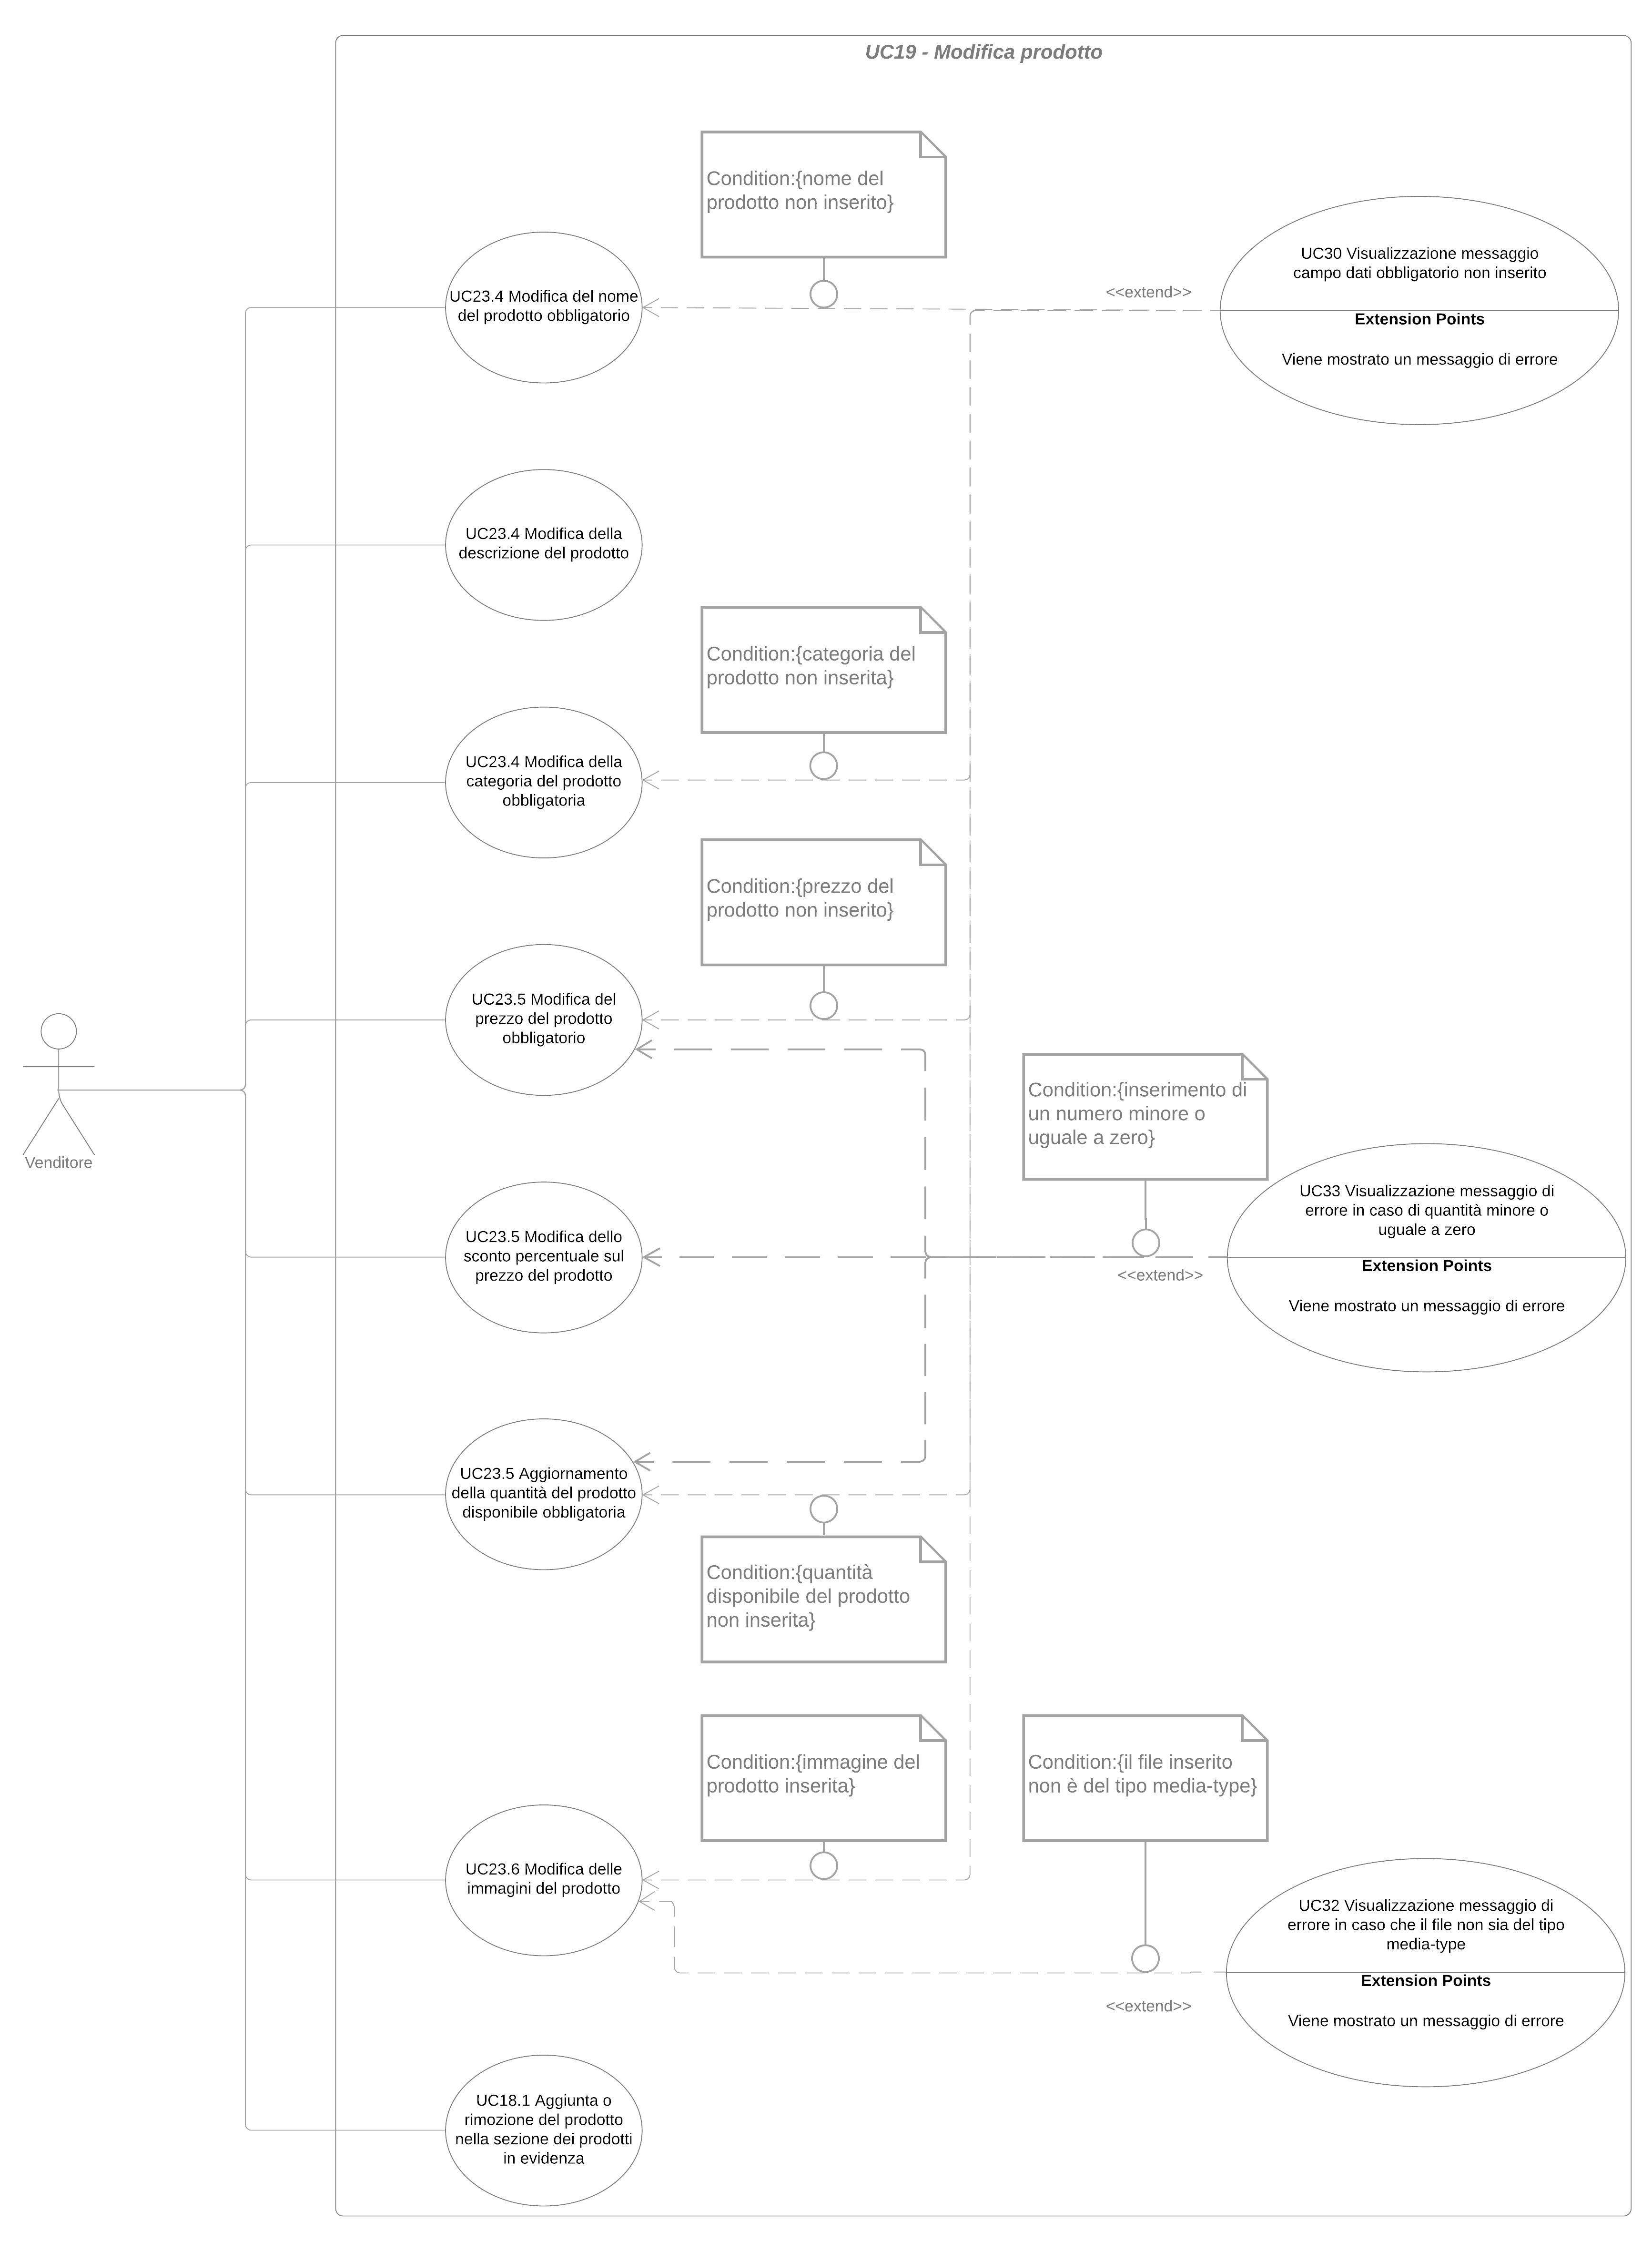
\includegraphics[scale=0.1]{Immagini/DiagrammiUC/UC19ModificaProdotto.png}
%     \caption{Diagramma di \actualUC: Modifica di un prodotto nella piattaforma da parte del venditore}
%     \label{fig:ModificaProdotto}
% \end{figure}

Il venditore modifica uno o più campi di un prodotto che è stato inserito nella piattaforma.
\begin{itemize}
    \item \textbf{Attori primari:} venditore;
    \item \textbf{Precondizione:} il venditore si trova nella PDP di un prodotto e clicca la funzionalità di modifica del prodotto selezionato;
    \item \textbf{Postcondizione:} il venditore ha modificato il prodotto con le modifiche compiute;
    \item \textbf{Scenario principale:} il venditore può compiere le seguenti azioni:
    \begin{itemize}
        \item (\actualUC.1) - Modifica del nome del prodotto;
        \item (\actualUC.2) - Modifica della descrizione del prodotto;
        \item (\actualUC.3) - Modifica delle categorie del prodotto;
        \item (\actualUC.4) - Modifica del prezzo del prodotto;
        \item (\actualUC.5) - Modifica dello sconto percentuale al prezzo del prodotto;
        \item (\actualUC.6) - Aggiunta di nuove foto del prodotto;
        \item (\actualUC.7) - Rimozione di foto del prodotto.
    \end{itemize}
    Il venditore conferma le modifiche compiute modificando in modo definitivo il prodotto selezionato;
    \item \textbf{Scenari alternativi:}
    \begin{enumerate}[label=\lett]
    	\item Il venditore non conferma le modifiche effettuate e perciò verranno scartate.
    \end{enumerate}
\end{itemize}

\resetSubUC
\subUC{Modifica del nome del prodotto}
Il venditore vuole modificare il nome del prodotto.
\begin{itemize}
    \item \textbf{Attori primari:} venditore;
    \item \textbf{Precondizione:} il venditore si trova nella schermata di modifica del prodotto;
    \item \textbf{Postcondizione:} il venditore ha modificato il nome del prodotto;
    \item \textbf{Scenario principale:} il venditore aggiorna il nome del prodotto selezionato;
    \item \textbf{Estensioni:}
    \begin{enumerate}[label=\lett]
    	\item Il venditore cancella il nome attuale del prodotto ed il campo dati risulta essere vuoto. In questo caso:
    	\begin{itemize}
    		\item (UC) - Viene visualizzato il messaggio di errore campo dati obbligatorio non inserito;
    		\item Viene fornita al venditore la possibilità di inserire un nuovo nome al prodotto selezionato.
    	\end{itemize}
    \end{enumerate}
\end{itemize}

\subUC{Modifica della descrizione del prodotto}
Il venditore vuole modificare la descrizione del prodotto.
\begin{itemize}
    \item \textbf{Attori primari:} venditore;
    \item \textbf{Precondizione:} il venditore si trova nella schermata di modifica del prodotto;
    \item \textbf{Postcondizione:} il venditore ha modificato la descrizione del prodotto;
    \item \textbf{Scenario principale:} il venditore modifica la descrizione del prodotto selezionato;
    \item \textbf{Estensioni:}
    \begin{enumerate}[label=\lett]
    	\item Il venditore cancella la descrizione attuale del prodotto ed il campo dati risulta essere vuoto. In questo caso:
    	\begin{itemize}
    		\item (UC) - Viene visualizzato il messaggio di errore campo dati obbligatorio non inserito;
    		\item Viene fornita al venditore la possibilità di inserire una nuova descrizione del prodotto selezionato.
    	\end{itemize}
    \end{enumerate}
\end{itemize}

\subUC{Modifica delle categorie del prodotto}
Il venditore modifica le categorie del prodotto.
\begin{itemize}
    \item \textbf{Attori primari:} venditore;
    \item \textbf{Precondizione:} il venditore si trova nella schermata di modifica del prodotto;
    \item \textbf{Postcondizione:} il venditore ha modificato le categorie del prodotto;
    \item \textbf{Scenario Principale:} il venditore modifica le categorie a cui fa parte il prodotto e può compiere le seguenti azioni:
    \begin{itemize}
        \item Aggiunta di una nuova categoria presa dalla lista di categorie disponibili;
        \item Rimozione di una categoria attualmente inserita.
    \end{itemize}
\end{itemize}

\subUC{Modifica del prezzo del prodotto}
Il venditore modifica il prezzo a cui vendere il prodotto.
\begin{itemize}
    \item \textbf{Attori primari:} venditore;
    \item \textbf{Precondizione:} il venditore si trova nella schermata di modifica del prodotto;
    \item \textbf{Postcondizione:} il venditore ha modificato il prezzo a cui vendere il prodotto;
    \item \textbf{Scenario principale:} il venditore modifica il prezzo a cui vendere il prodotto selezionato;
    \item \textbf{Estensioni:}
    \begin{enumerate}[label=\lett]
    	\item Il venditore cancella il prezzo attuale del prodotto ed il campo dati risulta essere vuoto. In questo caso:
    	\begin{itemize}
    		\item (UC) - Viene visualizzato il messaggio di errore campo dati obbligatorio non inserito;
    		\item Viene fornita la possibilità al venditore di inserire un nuovo prezzo per il prodotto selezionato.
    	\end{itemize}
    	\item Il venditore inserisce un nuovo prezzo minore o uguale a 0. In questo caso:
    	\begin{itemize}
    		\item (UC) - Verrà visualizzato il messaggio di errore in caso di prezzo minore o uguale a 0;
    		\item Viene fornita la possibilità al venditore di modificare il prezzo per il prodotto selezionato.
    	\end{itemize}
    \end{enumerate}
\end{itemize}

\subUC{Modifica dello sconto percentuale al prezzo del prodotto}
Il venditore modifica lo sconto percentuale da applicare al prezzo del prodotto.
\begin{itemize}
    \item \textbf{Attori primari:} venditore;
    \item \textbf{Precondizione:} il venditore si trova nella schermata di modifica del prodotto;
    \item \textbf{Postcondizione:} il venditore ha modificato lo sconto percentuale da applicare al prezzo del prodotto;
    \item \textbf{Scenario Principale:} il venditore modifica lo sconto percentuale da applicare al prezzo del prodotto selezionato;
    \item \textbf{Scenari alternativi:}
    \begin{enumerate}[label=\lett]
    	\item Nel caso in cui il venditore cancella lo sconto attuale senza inserirne uno di nuovo, non viene applicato alcuno sconto.
    \end{enumerate}
    \item \textbf{Estensioni:}
    \begin{enumerate}[label=\lett]
    	\item Il venditore inserisce uno sconto maggiore di 100\%. In questo caso:
		\begin{itemize}
			\item (UC) - Viene visualizzato il messaggio di errore in caso di sconto maggiore di 100\%;
			\item Viene fornita al venditore la possibilità di modificare lo sconto da applicare al nuovo prodotto.
		\end{itemize}
		\item Il venditore inserisce uno sconto minore di 0\%. In questo caso:
		\begin{itemize}
			\item (UC) - Viene mostrato un messaggio di errore che segnala lo sconto minore di 0\%;
			\item Viene fornita al venditore la possibilità di modificare lo sconto da applicare al nuovo prodotto.
		\end{itemize}
    \end{enumerate}
\end{itemize}

\subUC{Aggiunta di foto al prodotto}
Il venditore inserisce le foto relative al prodotto.
\begin{itemize}
    \item \textbf{Attori primari:} venditore;
    \item \textbf{Precondizione:} il venditore si trova nella schermata di modifica del prodotto;
    \item \textbf{Postcondizione:} il venditore ha inserito le foto relative al prodotto;
    \item \textbf{Scenario principale:} il venditore inserisce delle nuove foto relative al prodotto selezionato;
    \item \textbf{Estensioni:}
    \begin{enumerate}[label=\lett]
    	\item Il venditore seleziona un file che non è del tipo immagine. In questo caso:
		\begin{itemize}
			\item (UC) - Viene visualizzato il messaggio di errore il quale segnala che il file selezionato non è del tipo immagine;
			\item Viene fornita la possibilità al venditore di cambiare i file selezionati per il nuovo prodotto.
		\end{itemize}
		\item Il venditore cerca di inserire più del numero massimo di foto consentite relative ad un prodotto. In questo caso:
		\begin{itemize}
			\item (UC) - Viene visualizzato il messaggio di errore il quale segnala il tentativo di aggiunta di più del numero massimo di foto consentite relative ad un prodotto;
			\item Viene fornita la possibilità al venditore di rimuovere alcune foto selezionate per il nuovo prodotto da inserire.
		\end{itemize}
    \end{enumerate}
\end{itemize}

\subUC{Rimozione di foto dal prodotto}
Il venditore rimuove le foto relative al prodotto da aggiungere.
\begin{itemize}
    \item \textbf{Attori primari:} venditore;
    \item \textbf{Precondizione:} il venditore si trova nella schermata di modifica del prodotto;
    \item \textbf{Postcondizione:} il venditore ha rimosso le foto relative al prodotto;
    \item \textbf{Scenario principale:} il venditore rimuove le foto relative al prodotto attraverso i seguenti passi: 
    \begin{itemize}
        \item Seleziona la foto che vuole eliminare;
        \item Seleziona l'azione di eliminazione di quella specifica foto;
        \item Conferma la rimozione della foto selezionata.
    \end{itemize}
    \item \textbf{Estensioni:}
    \begin{enumerate}[label=\lett]
    	\item Il venditore cancella tutte le foto relative al prodotto. In questo caso:
    	\begin{itemize}
    		\item (UC) - Viene visualizzato il messaggio di errore campo dati obbligatorio non inserito;
    		\item Viene impedita la conferma delle modifiche al prodotto.
    	\end{itemize}
    \end{enumerate}
\end{itemize}

\UC{Aggiunta prodotto alla sezione dei prodotti in evidenza}
Il venditore aggiunge un prodotto alla sezione dei prodotti in evidenza presente nella vista principale.
\begin{itemize}
    \item \textbf{Attori primari:} venditore;
    \item \textbf{Precondizione:} il venditore si trova nella PDP del prodotto ed il prodotto non è stato aggiunto alla sezione dei prodotti in evidenza;
    \item \textbf{Postcondizione:} il prodotto viene aggiunto alla sezione dei prodotti in evidenza;
    \item \textbf{Scenario principale:} il venditore aggiunge un prodotto alla sezione dei prodotti in evidenza tramite la funzionalità adeguata che lo segnerà come in evidenza.
\end{itemize}

\UC{Rimozione prodotto dalla sezione dei prodotti in evidenza}
Il venditore rimuove un prodotto dalla sezione dei prodotti in evidenza presente nella vista principale.
\begin{itemize}
    \item \textbf{Attori primari:} venditore;
    \item \textbf{Precondizione:} il venditore si trova nella PDP del prodotto ed il prodotto è stato aggiunto alla sezione dei prodotti in evidenza;
    \item \textbf{Postcondizione:} il prodotto viene rimosso dalla sezione dei prodotti in evidenza; 
    \item \textbf{Scenario principale:} il venditore rimuove un prodotto dalla sezione dei prodotti in evidenza tramite la funzionalità adeguata che lo segnerà come non in evidenza.
\end{itemize}

\UC{Eliminazione prodotto}
\begin{figure}[H]
    \centering
    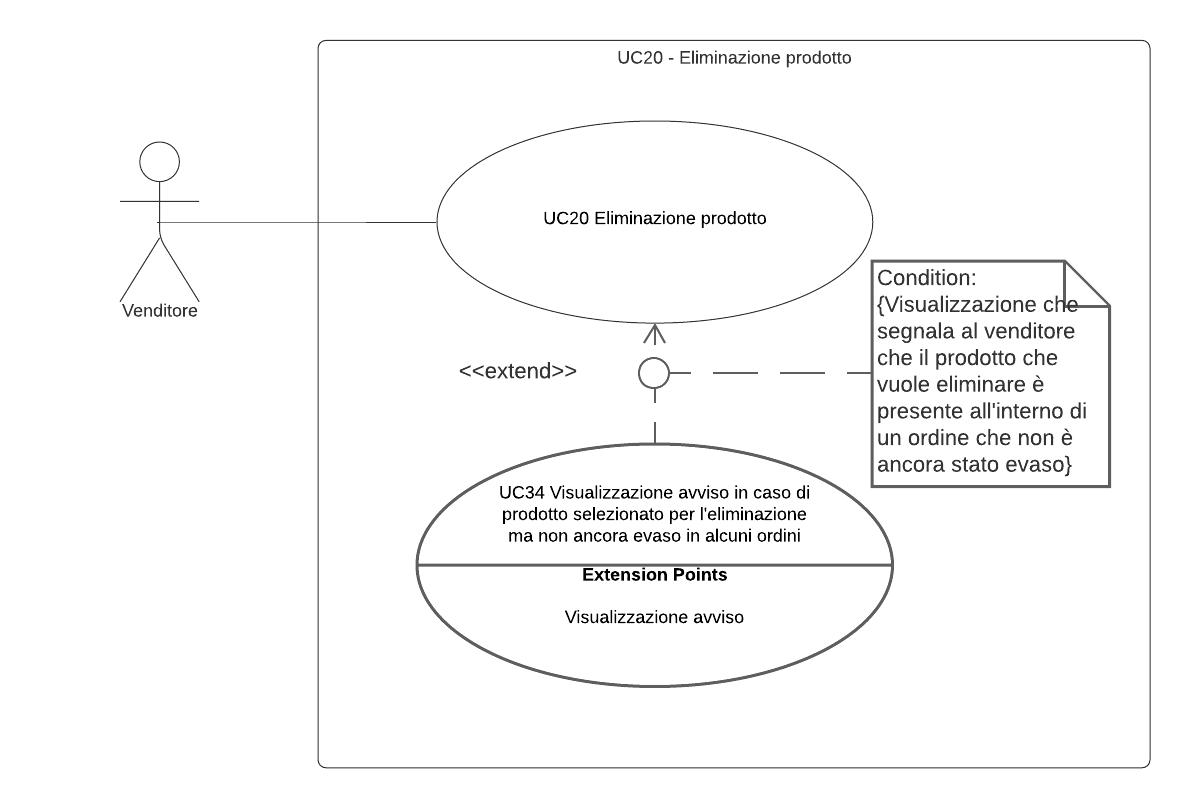
\includegraphics[width=\textwidth]{Immagini/DiagrammiUC/UC20EliminazioneProdotto}
    \caption{Diagramma di \actualUC: Eliminazione di un prodotto da parte del venditore} 
    \label{fig:EliminazioneProdotto}
\end{figure}

Il venditore vuole eliminare un prodotto precedentemente inserito.
\begin{itemize}
    \item \textbf{Attori primari:} venditore;
    \item \textbf{Precondizione:} il venditore si trova nella schermata della dashboard;
    \item \textbf{Postcondizione:} il venditore ha eliminato il prodotto selezionato;
    \item \textbf{Scenario Principale:} il venditore seleziona un prodotto dalla lista di quelli che ha inserito nella piattaforma, clicca sulla funzionalità per eliminarlo definitivamente e conferma l'eliminazione del prodotto selezionato. Di conseguenza:
    \begin{itemize}
    	\item Il prodotto viene rimosso da PDP, PLP, schermata principale, carrelli e dashboard;
    	\item Il prodotto rimane negli ordini già effettuati.
    \end{itemize}
	\item \textbf{Scenari alternativi:}
	\begin{enumerate}[label=\lett]
		\item Il venditore non conferma l'eliminazione del prodotto selezionato e di conseguenza questo rimarrà presente nella piattaforma.
	\end{enumerate}
    \item \textbf{Estensioni:}
    \begin{enumerate}[label=\lett]
    	\item Il venditore seleziona per l'eliminazione un prodotto che è stato ordinato ma non ancora pagato. In questo caso:
    	\begin{itemize}
    		\item (UC) - Viene visualizzato un messaggio di errore in caso di prodotto presente in un ordine non saldato;
    		\item Viene negato al venditore la possibilità di eliminare il prodotto selezionato.
    	\end{itemize}
    \end{enumerate}
\end{itemize}

\UC{Rifornimento prodotto}
Il venditore vuole rifornire un prodotto precedentemente inserito che sta per esaurire o è esaurito.
\begin{itemize}
    \item \textbf{Attori primari:} venditore;
    \item \textbf{Precondizione:} il venditore si trova nella schermata di amministrazione dei prodotti;
    \item \textbf{Postcondizione:} il venditore ha rifornito un prodotto;
    \item \textbf{Scenario principale:} il venditore seleziona un prodotto dalla lista di quelli che ha inserito nella piattaforma e preme sulla funzionalità per rifornirlo. Per completare il rifornimento deve svolgere i seguenti passi:
    \begin{itemize}
        \item Inserisce la quantità con cui rifornire il prodotto selezionato;
        \item Conferma il salvataggio della modifica.
    \end{itemize}
	\item \textbf{Scenari alternativi:}
	\begin{enumerate}[label=\lett]
		\item Il venditore inserisce la quantità con cui rifornire le scorte di un prodotto ma non conferma la modifica. In questo caso la quantità del prodotto non subisce alcuna modifica.
	\end{enumerate}
	\item \textbf{Estensioni:}
	\begin{enumerate}[label=\lett]
		\item Il venditore inserisce un valore inferiore a zero con cui rifornire le scorte di un determinato prodotto. In questo caso:
		\begin{itemize}
			\item (UC) - Viene visualizzato un messaggio di errore in caso di quantità minore a zero;
			\item Viene fornita al venditore la possibilità di modificare il valore inserito per rifornire il prodotto.
		\end{itemize}
	\end{enumerate}
\end{itemize}

\UC{Ricerca dei prodotti del venditore} 
Il venditore può cercare i prodotti dalla propria PLP attraverso delle parole.
\begin{itemize}
	\item \textbf{Attori primari:} venditore;
	\item \textbf{Precondizione:} il venditore ha selezionato la funzionalità per la ricerca;
	\item \textbf{Postcondizione:} il venditore visualizza i prodotti che contengono nella descrizione o nel nome, almeno una delle parole per le quali si è svolta la ricerca;
	\item \textbf{Scenario principale:} il venditore ha selezionato la funzione prevista per la ricerca. Dopo aver inserito le parole per individuare il prodotto, conferma la ricerca e viene aggiornata la PLP che mostra tutti i prodotti che hanno almeno una delle parole indicate nella descrizione o nel nome;
	\item \textbf{Scenari alternativi:}
	\begin{enumerate}[label=\lett]
		\item Il venditore ha svolto una ricerca in modo tale che questa non dia alcun risultato. In questo caso la PLP del venditore viene aggiornata mostrando il messaggio nessun prodotto trovato.
	\end{enumerate}
\end{itemize}

%%%%%%%%%%%%%%%%%%%%%%%%%%%%%%%%%%%%%%%%%%%%%%%%%%%%%%%%%%%%%%%%%%%%%%%%%%%%%%%%%%%%%%%%%%%%%%%%%%%%%%%%%%%%%%%%%%%%%%%%%%%%%%%%%%%%%%%%%%%%%%%%%%%%%%%%%%%%%

\UC{Filtraggio prodotti della PLP del venditore}
\begin{figure}[H]
	\centering
	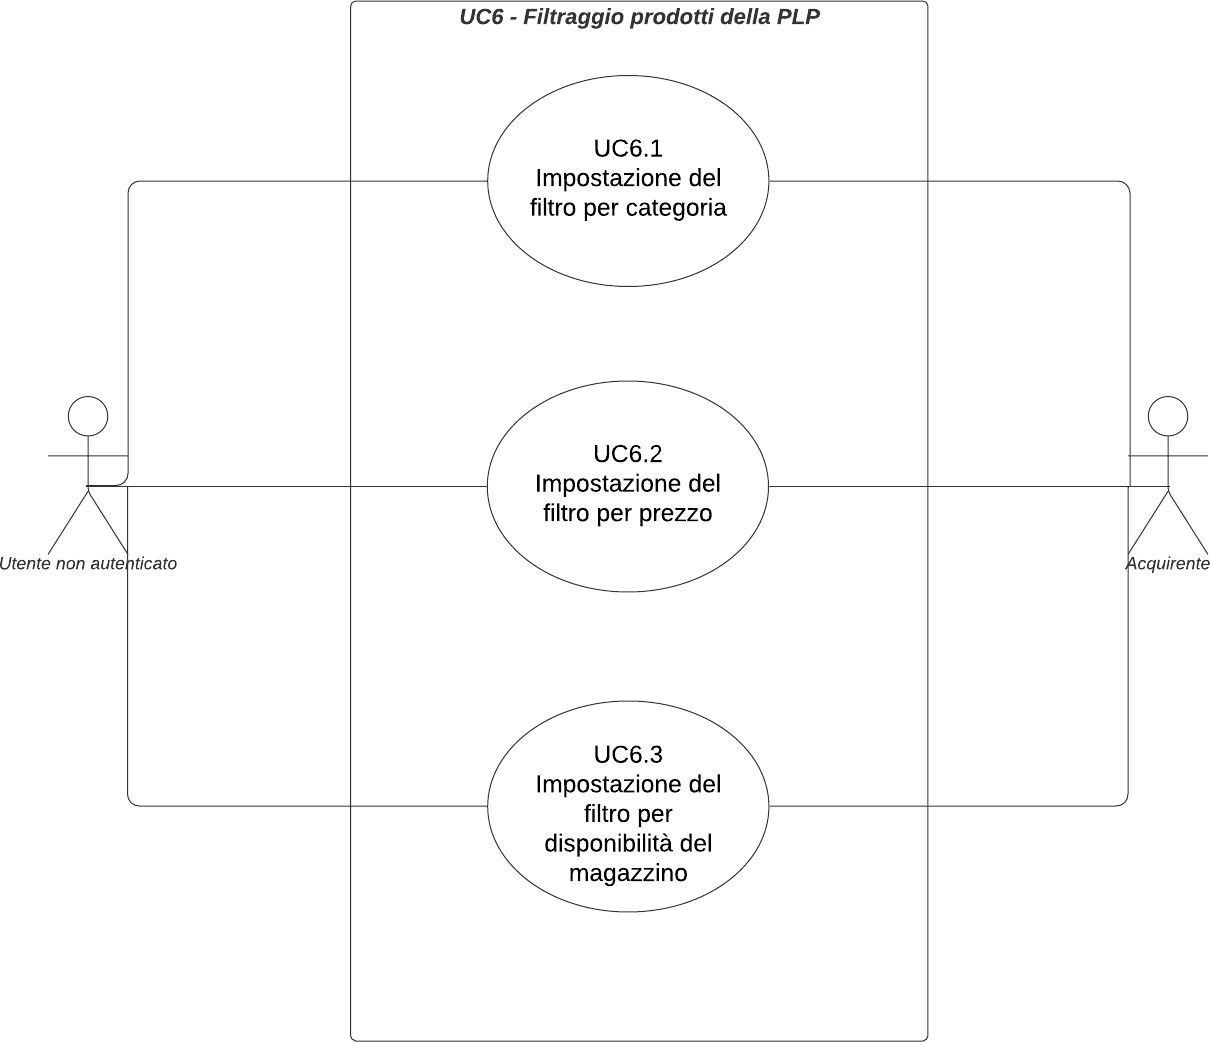
\includegraphics[scale=0.5]{Immagini/DiagrammiUC/UC6FiltraggioProdottiDellaPLP.png}
	\caption{Diagramma di \actualUC: Filtraggio dei prodotti della PLP} 
\end{figure}

Il venditore può filtrare i prodotti all'interno della PLP per categoria, prezzo, se è disponibile nel magazzino e se il prodotto è in evidenza o meno.
\begin{itemize}
	\item \textbf{Attori primari:} venditore;
	\item \textbf{Precondizione:} il venditore è nella PLP e ha impostato uno (o più) dei filtri disponibili per i quali cercare;
	\item \textbf{Postcondizione:} il venditore avrà a disposizione tutti i prodotti che soddisfano tutte le condizioni dei vari filtri impostati;
	\item \textbf{Scenario principale:} l'attore è nella PLP e ha impostato uno (o più) dei seguenti filtri:
	\begin{itemize}
		\item (\actualUC.1) - Impostazione del filtro per categoria;
		\item (\actualUC.2) - Impostazione del filtro per prezzo;
		\item (\actualUC.3) - Impostazione del filtro per disponibilità nel magazzino;
		\item (\actualUC.4) - Impostazione del filtro per prodotto in evidenza.
	\end{itemize}
	Di seguito la PLP verrà aggiornata con i prodotti che rispettano tutti i filtri applicati;
	\item \textbf{Scenari alternativi:}
	\begin{enumerate}[label=\lett]
		\item Il venditore ha impostato i filtri in modo tale che la ricerca con la loro combinazione non dia alcun risultato. In questo caso la schermata di riepilogo ordini viene aggiornata mostrando il messaggio nessun prodotto trovato.
	\end{enumerate}
\end{itemize}

\resetSubUC
\subUC{Filtro per categorie}
Il venditore può cercare i prodotti in base alla loro categoria, selezionando quelle di interesse tra tutte le categorie disponibili.
\begin{itemize}
	\item \textbf{Attori primari:} venditore;
	\item \textbf{Precondizione:} il venditore è nella PLP e ha selezionato una (o più) categorie tra quelle disponibili per quali filtrare;
	\item \textbf{Postcondizione:} il venditore visualizzerà nella PLP i prodotti che appartengono ad almeno una delle categorie selezionate;
	\item \textbf{Scenario principale:} il venditore è nella PLP e ha selezionato una (o più) categorie tra quelle disponibili per quali filtrare e di seguito verranno visualizzati i prodotti che appartengono ad almeno una delle categoria selezionate;
	\item \textbf{Scenari alternativi:}
	\begin{enumerate}[label=\lett]
		\item Se il venditore non imposta il seguente filtro, allora verranno visualizzati tutti i prodotti a prescindere della categoria.
	\end{enumerate}
\end{itemize}

\subUC{Filtro per prezzo}
Il venditore può cercare i prodotti in base al loro prezzo.
\begin{itemize}
	\item \textbf{Attori primari:} venditore;
	\item \textbf{Precondizione:} il venditore è nella PLP e ha selezionato uno tra gli intervalli di prezzo disponibili oppure ha inserito un intervallo personalizzato;
	\item \textbf{Postcondizione:} il venditore visualizzerà nella PLP i prodotti filtrati in base all'intervallo di prezzo selezionato;
	\item \textbf{Scenario principale:} il venditore seleziona l'intervallo di prezzo, oppure ne fornisce uno personalizzato per filtrare i prodotti, e verranno visualizzati i prodotti che entrano nell'intervallo di prezzo selezionato;
	\item \textbf{Scenari alternativi:}
	\begin{enumerate}[label=\lett]
		\item Se il venditore non imposta il seguente filtro, allora verranno visualizzati tutti i prodotti a prescindere dal prezzo.
	\end{enumerate}
\end{itemize}

\subUC{Filtro per disponibilità nel magazzino}
Il venditore può cercare i prodotti in base alla loro disponibilità in magazzino.
\begin{itemize}
	\item \textbf{Attori primari:} venditore;
	\item \textbf{Precondizione:} il venditore è nella PLP e ha attivato il filtro per disponibilità in magazzino;
	\item \textbf{Postcondizione:} il venditore visualizzerà nella PLP i prodotti che sono disponibili in magazzino;
	\item \textbf{Scenario principale:} il venditore ha attivato il filtro per disponibilità in magazzino e verranno visualizzati i prodotti che sono disponibili in magazzino;
	\item \textbf{Scenari alternativi:}
	\begin{enumerate}[label=\lett]
		\item Se il venditore non imposta il seguente filtro, allora verranno visualizzati tutti i prodotti a prescindere dalla loro disponibilità.
	\end{enumerate}
\end{itemize}

\subUC{Filtro per prodotto in evidenza}
Il venditore può cercare i prodotti in base alla loro caratteristica di trovarsi in evidenza o meno nella piattaforma.
\begin{itemize}
	\item \textbf{Attori primari:} venditore;
	\item \textbf{Precondizione:} il venditore è nella PLP e ha attivato il filtro per prodotto in evidenza;
	\item \textbf{Postcondizione:} il venditore visualizzerà nella PLP i prodotti che sono in evidenza;
	\item \textbf{Scenario principale:} il venditore ha attivato il filtro per prodotto in evidenza e verranno visualizzati i prodotti che sono in evidenza all'interno del sistema;
	\item \textbf{Scenari alternativi:}
	\begin{enumerate}[label=\lett]
		\item Se il venditore non imposta il seguente filtro, allora verranno visualizzati tutti i prodotti a prescindere dalla loro caratteristica di trovarsi in evidenza.
	\end{enumerate}
\end{itemize}